%%!TEX root = dissertation.tex
\setcounter{chapter}{3}

\chapter{The structure of voice onset time variation in bilingual long-lag stop categories}\label{Uniformity}

\section{Introduction}\label{ch4:sec:intro}

A consequence of bilingualism is that individuals must navigate segment inventories that exist in a shared phonetic space, in which categories may or may not share aspects of their mental representations \citep{flege_2021_slmr}. One of the primary goals in this chapter is to address what languages share, if anything, in the mental representation of speech sound categories. The idea of representation is intended here in the manner typically meant by psycholinguists \citep[e.g.,][]{llompart_2018_acoustic}, exemplar theory proponents \citep[e.g.,][]{amengual_2018_laterals}, and \citet{flege_2021_slmr} in the revised Speech Learning Model (SLM-r). \citeauthor{flege_2021_slmr} describe the units of a multilingual segment inventory as categories comprising input distributions of exemplars: ``the sensory stimulation associated with...speech sounds that are heard and seen during production by others...in meaningful conversations'' \citep[][p. 32]{flege_2021_slmr}. So, if sound categories from different languages exist in the same phonetic space and are represented by distributions of exemplars, how, then, can the extent to which languages share representation(s) be assessed? Much like Chapter \ref{}, the approach here is one of elucidating the structure of variation. 

There are many pieces to this puzzle, and the literature has already addressed some of them. The introduction to this chapter proceeds as follows---section \ref{ch4:sec:links} addresses which sound categories are candidates for shared representation in the first place. Section \ref{ch4:sec:cli} briefly summarizes the relevant crosslinguistic influence literature, addressing assimilation, dissimilation, and how they reflect on the idea of shared representation. Section \ref{ch4:sec:uniformity} identifies a limitation of the existing paradigms in crosslinguistic influence and proposes adapting the uniformity framework as a way to fill the gap. This framework offers a way to interpret the structure of variation for a given acoustic dimension. Section \ref{ch4:sec:rqs} introduces the focus of this particular study---long-lag stops in Cantonese and English---and outlines the specific research questions and hypotheses.

\subsection{Identifying ``links'' across languages}\label{ch4:sec:links}

At first glance, the best candidates for shared representation are sound categories discussed as being ``linked'' together. Yet, the definition of links can be frustratingly vague in the multilingualism literature. In a handbook chapter on bilingual phonetics and phonology, \citet{simonet_2016_bilingualism} describes ``links or connections of one sort or another between the phonetic categories'' (p. 10). While vague, links nonetheless represent a crucial concept. In the most basic sense, links are defined by the behavior they account for---they exist between sound categories that exert influence on one another under some set of circumstances. Links behave dynamically, as as such,  \citeauthor{simonet_2016_bilingualism} also notes that ``these connections...are transiently strengthened in contexts that induce the activation of both languages and inhibited in contexts that favor the use of only one of the languages'' \citeyearpar[][p. 10]{simonet_2016_bilingualism}. Arguably, the links must exist because crosslinguistic influence can be observed. While there may be alternative explanations (i.e., global influence), the concept of links is widely used in accounting for bilinguals' behavior. 

\citet{flege_2021_slmr} expand on links in the SLM-r, providing a framework for predicting which sound categories will be linked together. The proposal is simple---namely, sound categories will be linked to the closest category in the other language. Determining which categories pair up, however, remains an empirical challenge from the perspective of speech production, and as a result, \citet{flege_2021_slmr} rely on perceptual metrics. The reason for this challenge is because perception and production do not always line up neatly. \citeauthor{flege_2021_slmr} assert that similarity ``must be assessed perceptually rather than acoustically because acoustic measures sometimes diverge from what listeners perceive'' \citeyearpar[][p. 33]{flege_2021_slmr}. This assertion is echoed in an overview chapter on crosslinguistic segment similarity, where \citet{chang_2015_similarity} argues that in accounting for behavior, similarity is best captured abstractly. \citeauthor{chang_2015_similarity} states that crosslinguistic influence at the segmental level tends to occur between sounds that share ``(1) similar positions in the respective phonemic inventories (when considering the contrastive feature oppositions---or, more broadly, the `relative phonetics'---of the sounds in relation to other sounds in the inventory), and (2) similar distributional facts'' \citeyearpar[][p. 201]{chang_2015_similarity}. This approach to similarity emphasizes a general role for abstraction but does not necessarily invite a formal phonological analysis. Developing such an analysis would likely constitute a dissertation in itself---\citet{mielke_2012_similarity} highlights the challenges of applying phonological features across languages, given the sheer variety of phonetics-phonology mappings in the world's languages. 

While \citet{flege_2021_slmr} and \citet{chang_2015_similarity} take different approaches, perceptual ratings and relative phonetics accomplish a similar goal---they account for abstraction and nonlinearity in listeners' mental representations. In sum, abstract similarity seems to be a prerequisite for the emergence of a link between two sound categories, given how it does a better job of accounting for when and where crosslinguistic influence occurs. The presence of abstract similarity, however, does not address what happens next. It does not entail any particular outcome, and it does not directly address how representation is structured for the sound categories in question. 

\subsection{Crosslinguistic influence and representation}\label{ch4:sec:cli}

The next step in the puzzle is understanding what happens to linked sound categories. The SLM-r outlines two primary outcomes for sound categories in a shared system---assimilation and dissimilation \citep{flege_2021_slmr}. Assimilation is a merging of phonetic properties and arguably occurs when bilinguals and learners do not perceive a difference between two categories. Dissimilation, then, is the reverse---a diverging of phonetic properties that occurs when a difference is perceived. Notably, these processes need not impact all phonetic properties in the same way. For example, in a study of coronal stops produced by simultaneous French-English bilinguals, \citet{sundara_2006_production} found that bilinguals differentiated languages on voice onset time (VOT) and the standard deviation of burst frequency but not on the other spectral moments that monolinguals did differentiate. This study illustrates convergence on some but not all properties. 

The motivation for these outcomes arises from two simple constraints from the productive and perceptual systems. Effectively, don't get too close to each other in perception, and don't get too complicated in production \citep{guion_2003_systems, lindblom_1988_universals, flege_2021_slmr}. These constraints lead SLM-r to posit that proximity leads to instability, even if what counts as close remains unclear, and that the outcome of instability is assimilation and dissimilation. Considering how bilinguals are fully capable of maintaining subtle distinctions for similar sound categories across languages \citep[e.g.,][]{sundara_2006_production, casillas_2021_interlingual}, this is not a trivial point to make. It may thus be more appropriate in the case of early bilinguals to also consider contrast maintenance alongside dissimilation. 

By following what SLM-r posits, a relatively simple account is that dissimilation for similar sound categories would lead to distinct representations of those categories. A similarly straightforward account is that assimilation leads to a shared representation. The picture is complicated, however, by the idea of imperfect assimilation and what \citeauthor{flege_2021_slmr} term \textit{composite categories}. In the SLM-r, if sounds from two languages are phonetically too close to each other, they will remain linked in a composite category "defined by the statistical regularities present in the combined distributions of the perceptually linked...sounds." \citep[][p. 41]{flege_2021_slmr}. This scenario might be characterized as imperfect or partially shared representation, where certain dimensions are kept apart and others overlap. For example, the place of articulation may be shared across languages even if VOT differs. Alternatively, this lack of clear-cut examples of assimilation in the literature may instead indicate that assimilation and dissimilation might be better cast as ends of a spectrum for a gradient, context-sensitive phenomenon. This re-conceptualization makes room for things like contrast maintenance and composite categories.

There are a few potential reasons for the lack of clear-cut assimilation. First, true assimilation might just be rare in bilingual speech. This reason is supported by a recent meta-analysis of crosslinguistic influence for Spanish and English initial stop consonants \citep{casillas_2021_interlingual}. In this environment, English long-lag stops and Spanish short-lag stops are linked to one another \citep{}. \citeauthor{casillas_2021_interlingual} found that early bilinguals did not produce ``compromise'' stop categories. That is, early Spanish-English bilinguals did not produce VOT was somehow intermediate to canonical productions by monolinguals of either language. Instead, the production of each category was influenced by task demands and factors such as social context. So while some assimilation occurs, it is far from the only process. This finding echoes arguments made by \citet{bullock_2009_sociophonetics} on the sophistication and control that bilinguals exert over their possible forms. So while there is clear evidence of a link between the two sounds, there is no compromise category. Instead, bilinguals produce a wide range of forms appropriate to and influenced by different contexts. Without considering task and context factors, it is perhaps not surprising that the two sound categories masquerade as a single composite category. 

A second reason for the rarity of complete assimilation arises from the experimental and corpus-based approaches typically used to study crosslinguistic influence. In these approaches, the ability to examine crosslinguistic influence for any given pair of sounds hinges on the presence of an observable difference under some set of conditions. I posit that for this reason, most prior work in crosslinguistic influence has focused on sounds that are phonologically similar (i.e., abstract, relative phonetics) yet phonetically distinct. A common example of this arises from languages that differ in their initial stop voicing contrasts. North American English contrasts long- and short-lag stops in initial position; conversely, Spanish contrasts short-lag and prevoiced initial stops. Despite the clear difference in how the languages encode a laryngeal timing contrast, there is strong evidence for a crosslinguistic link between English long-lag and Spanish short-lag stops \citep{casillas_2021_interlingual, fricke_2016_phonetic, goldrick_2014_switching, bullock_2009_sociophonetics, olson_2016_transfer}. 

These studies demonstrate phonetic convergence---or variable assimilation---in two ways. First, VOT is shorter for English initial stops produced by bilinguals when compared to monolingual control groups. This result is attributed to the influence on English long-lag stops from the short-lag category in the other language \citep{olson_2016_transfer}. Similarly, French-English bilinguals are more likely to produce lead voicing in initial English voiced stops compared to English monolinguals \citep{sundara_2006_production}. Second, evidence of crosslinguistic influence can also come from comparing bilinguals to themselves across different circumstances. For example, \citet{fricke_2016_phonetic} use a spontaneous speech corpus to demonstrate that Spanish-English bilinguals produce shorter, more Spanish-like VOT in the lead up to an English-to-Spanish code switch \citep{fricke_2016_phonetic}. While this body of work makes the presence of a link clear, it also highlights that there are distinct aspects of how these sound categories are represented in the bilingual mind \citep{casillas_2021_interlingual}. In the SLM-r, these examples might be considered composite categories. Alternatively, they might be examples of contrasts being maintained in the face of proximity.

In any case, this focus presents a conundrum. By using methods where observing similarity hinges on the ability to detect a difference, researchers preemptively exclude the best candidates for shared representation---those that share both abstract and acoustic similarity. One example comparing highly similar sound categories in the early bilingualism literature comes from a lab-based study of Mandarin-English bilingual children \citep{yang_2019_vot}. The authors found that highly proficient bilingual 5 to 6-year-olds produced equivalent VOT for Mandarin and English long-lag stops, even though the monolingual comparison groups were consistently different. \citeauthor{yang_2019_vot}'s result suggests that the difference is either too small to maintain or that 5 to 6-year-old children have not yet mastered it. These claims should be tempered, however, as \citet{yang_2019_vot} did not control for language mode, and adult bilingual behavior was not considered. 

% Add in \citep{macleod_2005_vot, lein_2016_vot} discussion
%

Despite some inroads, there is nonetheless a distinct paucity of work examining highly phonetically similar speech sounds across languages, even when such a connection would make sense. A recent study of crosslinguistic influence in Cantonese-English bilinguals compares English long-lag and Cantonese short-lag stops in the context of a language switching paradigm \citep{tsui_2019_switching}. While this comparison reflects the need for stimuli to be acoustically distinct beforehand, it glosses over the fact that both languages contrast short-lag and long-lag VOT in initial position. The best candidates for links---and accompanying crosslinguistic influence---should be the long-lag stops in each language. The null result with balanced bilinguals is thus unsurprising. I do not mean to suggest that the \citep{tsui_2019_switching} would have gotten more insightful results by comparing Cantonese long-lag stops to English long-lag stops. Instead, I aim to highlight the design constraints of the paradigms used in crosslinguistic influence research. Such methods are better suited for detecting dissimilation or contrasts that have been maintained. Conversely, methods for assessing assimilation must not rely on the presence of detectable acoustic differences.

To summarize, most work in crosslinguistic influence has focused on phonologically similar yet phonetically distinct pairs of segments, which are not strong candidates for shared mental representation (as defined at the beginning of this chapter). This focus of this work on telling sounds apart is likely a result of commonly-used paradigms requiring differences to detect influence and the possibility that assimilation may be rare in early bilingual speech. Additionally, comparisons of categories that already exhibit both abstract and phonetic similarity may be taken for granted and not considered an interesting problem to focus on, despite the nature of the mental representation of sound categories being a key focus in psycholinguistics \citep{samuel_2020_resist}. In this sense, studying interactions between systems in bilingual speech offers yet another window into linguistic processing \citep{fricke_2019_bilingualism}. In the interest of understanding mental representation, the best category candidates would be the hardest to distinguish using surface forms in the first place. 

\subsection{Adapting the uniformity framework}\label{ch4:sec:uniformity}

The study described in this chapter focuses on assessing whether phonetically similar sounds share representation or not. Unlike prior work that tells sound categories apart, this chapter aims to tell sound categories together---that is, does a single category deploy to each language, or does each language have its own version. Testing directly for shared structure in this way means that the set of methods that rely on detecting and modulating differences is not appropriate. To this end, I extend the articulatory uniformity framework to the study of multilingual segment inventories. 

Articulatory uniformity is conceptualized as a constraint on within-talker phonetic variation, in which articulatory gestures or phonological primitives are implemented systematically in speech production \citep{chodroff_2017_structure, faytak_2018_uniformity, menard_2008_invariance}. The core idea of the articulatory uniformity framework is that phonetic variation is highly structured. While \citet{chodroff_2017_structure} draw tight connections between uniformity and phonological features, \citet{faytak_2018_uniformity} emphasizes how talkers learn and reuse articulatory gestures. The articulatory account builds on earlier work by \citet{menard_2008_invariance}, who argue that the stability of the first formant in French vowel production is best accounted for by stability in the tongue height gesture. While the theoretical account varies somewhat by author, there is nothing to suggest that such accounts are incompatible. That is, both articulatory and phonological explanations are likely valid. Given the focus of this chapter on phonetic and psycholinguistic accounts of category formation and representation, the articulatory account is perhaps more appropriate. % something here from Lieberman 1988?? on stability and quantal regions?

In this light, if a set of segments share an attribute, then talkers should implement the segments with the same phonetic target or articulatory gesture---which may or may not have an acoustic consequence. This systematicity has been observed for in vowel height \citep{menard_2008_invariance}, tongue shape \citep{faytak_2018_uniformity}, fricative peak frequency, and stop consonant VOT \citep{chodroff_2017_structure}. In the case of VOT in particular, the relationship between a laryngeal gesture and its acoustic consequence is clear. This allows for the extension of \citeauthor{menard_2008_invariance}'s \citeyearpar{menard_2008_invariance} argument regarding F1 and tongue height to VOT and its corresponding laryngeal gesture. Reusing the gesture across sounds that share the relevant attribute ``may simplify the somatosensory feedback needed to control the speech task`` \citep[][p. 26]{menard_2008_invariance}. In simple terms, reusing gestures is easier than the alternative in the case of high vowels. I posit that the same argument could easily be extended for long-lag stops. 

Findings for stop consonant within-language uniformity appear to be quite robust. \citet{chodroff_2017_structure} report consistent results across a lab study based on reading a list of CVC and a corpus study using connected read speech. \citet{chodroff_2019_l2} replicate the uniformity findings for stop consonants with read speech samples from 140 non-native English speakers in the ALLSSTAR corpus \citep[wide range of native languages][]{bradlow_2011_allsstar}. While \citet{chodroff_2019_l2} found a greater degree of between-talker variability with non-native speakers compared to the prior monolingual work, the within-talker structure was robust. However, the uniformity framework has not yet been extended to early bilingual speech, in particular as a mechanism for comparing how bilinguals produce phonetically similar sounds in each of their languages. Extending the framework in this way follows the framing of uniformity as arising from articulatory reuse \citep{faytak_2018_uniformity}. 

\subsection{Long-lag stops in Cantonese and English}\label{ch4:sec:rqs}

English and Cantonese initial long-lag stops are strong candidates for shared underlying representation because they exhibit both acoustic and relative phonetic similarity, akin to the difference for Mandarin and English in \citet{yang_2019_vot}. Consider the initial stop [k\textsuperscript{h}] with a mean VOT of 80 ms in American English \citep{lisker_1964_vot} and 91 ms in Hong Kong Cantonese \citep{clumeck_1981_cantonese}. While these values are objectively different---though based on small sample sizes---it seems that using the same laryngeal timing gesture would be advantageous given the small difference across monolingual populations that may or may not be perceptible. While there is a limited amount of work documenting Cantonese long-lag VOT, descriptive work casts it as generic long-lag aspiration similar to English \citep{matthews_2013_cantonese, bauer_1997_cantonese, chan_2000_english,mielke_2018_voice}. For example, \citet{matthews_2013_cantonese} describe initial stops in both English and Cantonese as voiceless and aspirated, even though they differ in their phonological features. 
 
While the presence of articulatory reuse within Cantonese and across languages remains an empirical question, it follows from the finding that bilingual Mandarin-English children did not distinguish between languages in VOT \citep{yang_2019_vot}. Following the predictions of the SLM-r \citep{flege_2021_slmr}, this work suggests that long-lag items of minimally distinct VOT would assimilate or dissimilate but not be stable in such close proximity. 

Thus, the present study asks: Do Cantonese-English bilinguals uniformly produce long-lag stops within and across each of their languages? Leveraging the methodology from Chodroff and colleagues \citep{chodroff_2017_structure, chodroff_2018_predictability, chodroff_2019_l2} allows for a new perspective on the structure of variation and nature of representation in bilinguals. It also facilitates the study of phonetically similar speech sounds in ways that other paradigms do not. As may be clear from the framing of the introduction, the hypothesis was that bilinguals would indeed exhibit crosslinguistic uniformity.

\section{Methods}

\subsection{Corpus}
This study uses conversational interview recordings from the SpiCE corpus described in Chapter 2. As a reminder, the corpus comprises recordings of 34 early Cantonese-English bilinguals in both languages. The analysis in this chapter builds on the force-aligned phone transcripts. Please refer to Chapter \ref{ch:Corpus} for additional information about the talkers. 

\subsection{Segmentation \& measurement}

All instances of prevocalic word-initial /p t k/ were identified from the SpiCE corpus' force-aligned Praat TextGrid transcripts. For English, only items with initial stress were included in the initial sample \citep{lisker_1967_some}---this means the extremely high-frequency English word ``to'' was excluded, as was the case in \citet{chodroff_2017_structure}. Code-switches out of the interview's primary language were not aligned, and as a result, they do not appear in the phone tier of the TextGrids. This limitation of forced alignment means that Cantonese /p t k/ were only considered if they occurred in the Cantonese interviews, and likewise for English. The initial total count across talkers and languages included 10,428 tokens. 

While forced alignment performed reasonably well, anecdotally speaking, VOT estimates were refined using AutoVOT \citep{keshet_2014_autovot}---a command-line software tool that facilitates automated measurement of positive VOT. AutoVOT identifies the onset and offset of positive VOT within a specified window and with a minimum duration, as determined by the user. Here, the minimum allowed VOT was set to 15 ms. This value was selected as the stops under consideration are all long-lag stops, and aspiration values under 15 ms are typical of short-lag stops \citep{lieberman_1988_speech}. The window used with AutoVOT was defined as the force-aligned segment boundaries plus or minus 31 ms. If stops were too close for a 31 ms buffer, the onset of the second stop's window was set as the offset of the preceding window, as TextGrids do not permit overlapping intervals and AutoVOT uses the full TextGrid.  

After running AutoVOT, instances of /p t k/ were subjected to exclusionary criteria to catch errors. Items were excluded if there was substantial enough misalignment such that the AutoVOT offset did not fall within the original force-aligned boundaries of the word ($n=567$), if the previous word was unknown (i.e., unintelligible or in a different language; $n=263$), if VOT was equal to the minimum value of 15 ms ($n=446$), or if items had a VOT more than 2.5 standard deviations above the grand mean ($>129.5$ ms; $n=191$).

Of the initial sample, 14.1\% was excluded, resulting in 8,961 stops, summarized in Table \ref{ch3:tab:counts}. Talkers had a median of 97 Cantonese stops (range: 54-194) and 150.5 English stops (range: 73-540). While Cantonese stops were culled at a slightly higher rate (43\% of initial sample, 38\% of final sample), the higher number of English stops is likely due primarily to lexical distributional reasons. Additionally, English has a greater number of highly frequent /k/-initial word types, while Cantonese /p/ occurs in fewer, less frequent word types in the final sample ($n=60$, max frequency of 97) than English ($n=158$, max frequency of 215).

\begin{table}[htb]
  \caption{The number of stop token for each language and sound category.}
  \label{ch3:tab:counts}
  \centering
  \begin{tabular}{llll}
    \toprule
    \textbf{Language}  & \textbf{/p/} & \textbf{/t/} & \textbf{/k/} \\
    \midrule
    Cantonese & 374          & 1373         & 1688         \\
    English   & 1035         & 1336         & 3155   \\
    \bottomrule     
  \end{tabular}
\end{table}

\section{Analysis \& Results}
The articulatory uniformity framework offers strong theoretical grounds for interpreting the structure of VOT variation within and across talkers. This analysis qualifies and quantifies that structure from a few different perspectives. Section \ref{ch4:sec:ordrel} describes the ordinal relationship between each of the segments across talkers and languages. Section \ref{ch4:sec:correlations} reports on a series of pairwise correlations of talker means for each of the three segments in each language. Lastly, Section \ref{ch4:sec:lmem} comprises the results of a linear mixed effects model aimed at elicidating the role of language while accounting for variables known to impact VOT.

% methods revised up to here

\subsection{Ordinal relationships}\label{ch4:sec:ordrel}

Prior work with lab and read speech strongly suggests an expected ordinal relationship for VOT across places of articulation, in which /p/ is consistently shorter than /k/ and /t/ tends to fall in the middle. The argument for this widely attested pattern is based on vocal tract aerodynamics and articulatory constraints \citep{cho_1999_vot}. One of the major contributions of \citet{chodroff_2017_structure} is that these relationships are tighter than would be expected from a purely ordinal perspective. While ordinal relationships are a starting place, they represent just one piece of the puzzle. 

The results suggest that \textit{puzzle} is an appropriate characterization, as talkers largely did not adhere to the expected order. While there is some reason to expect coronals not to pattern accordingly, the relationship between /p/ and /k/ is inconsistent across talkers. Table \ref{tab:ordrel} reports the proportion of talkers whose mean VOT values followed the expected /p/ $<$ /t/ $<$ /k/ relationships. Prior work with connected speech reports rates of adherence in the 80-90\% range, except for English /t/ $<$ /k/ being drastically lower for native English speakers \citep{chodroff_2019_l2}. While the English /t/ $<$ /k/ comparison is remarkably low here (6\%), only English /p/ $<$ /t/ (82\%) falls in the range that prior work suggests. This lack of adherence is apparent in the relative ordering or markers in Figures \ref{ch4:fig:ordrelvf} and \ref{ch4:fig:ordrelvm}, which depict the mean and standard error of VOT for each segment, language, and talker. In many cases, the standard errors for the different segments in a given talker's panel overlap, indicating that strict ordering may not be appropriate here. Additionally, talkers do not appear to be consistent across languages. For example, talker VF19B in Figure \ref{ch4:fig:ordrelvf} exhibits a clear  /p/ $<$ /t/ $<$ /k/ relationship in Cantonese, but a clear /p/ $<$ /k/ $<$ /t/ relationship in English. 

\begin{table}[hb!]
\caption{Proportion of talker means that adhered to expected ordinal relationship for VOT: /p/ $<$ /t/ $<$ /k/ VOT durations. Note that talker VM25A has no instances of Cantonese /p/ in the final sample.}
  \label{tab:ordrel}
  \centering
  \begin{tabular}{lllll}
    \toprule
    \textbf{Language} & \textbf{p$<$t} & \textbf{t$<$k} & \textbf{p$<$k} & \textbf{n} \\
    \midrule
    Cantonese	& 0.24	& 0.61	& 0.39	& 33 \\
    English	    & 0.82	& 0.06	& 0.47	& 34 \\
    \bottomrule
  \end{tabular}
\end{table}

\begin{figure}[htbp]
  \begin{center}
  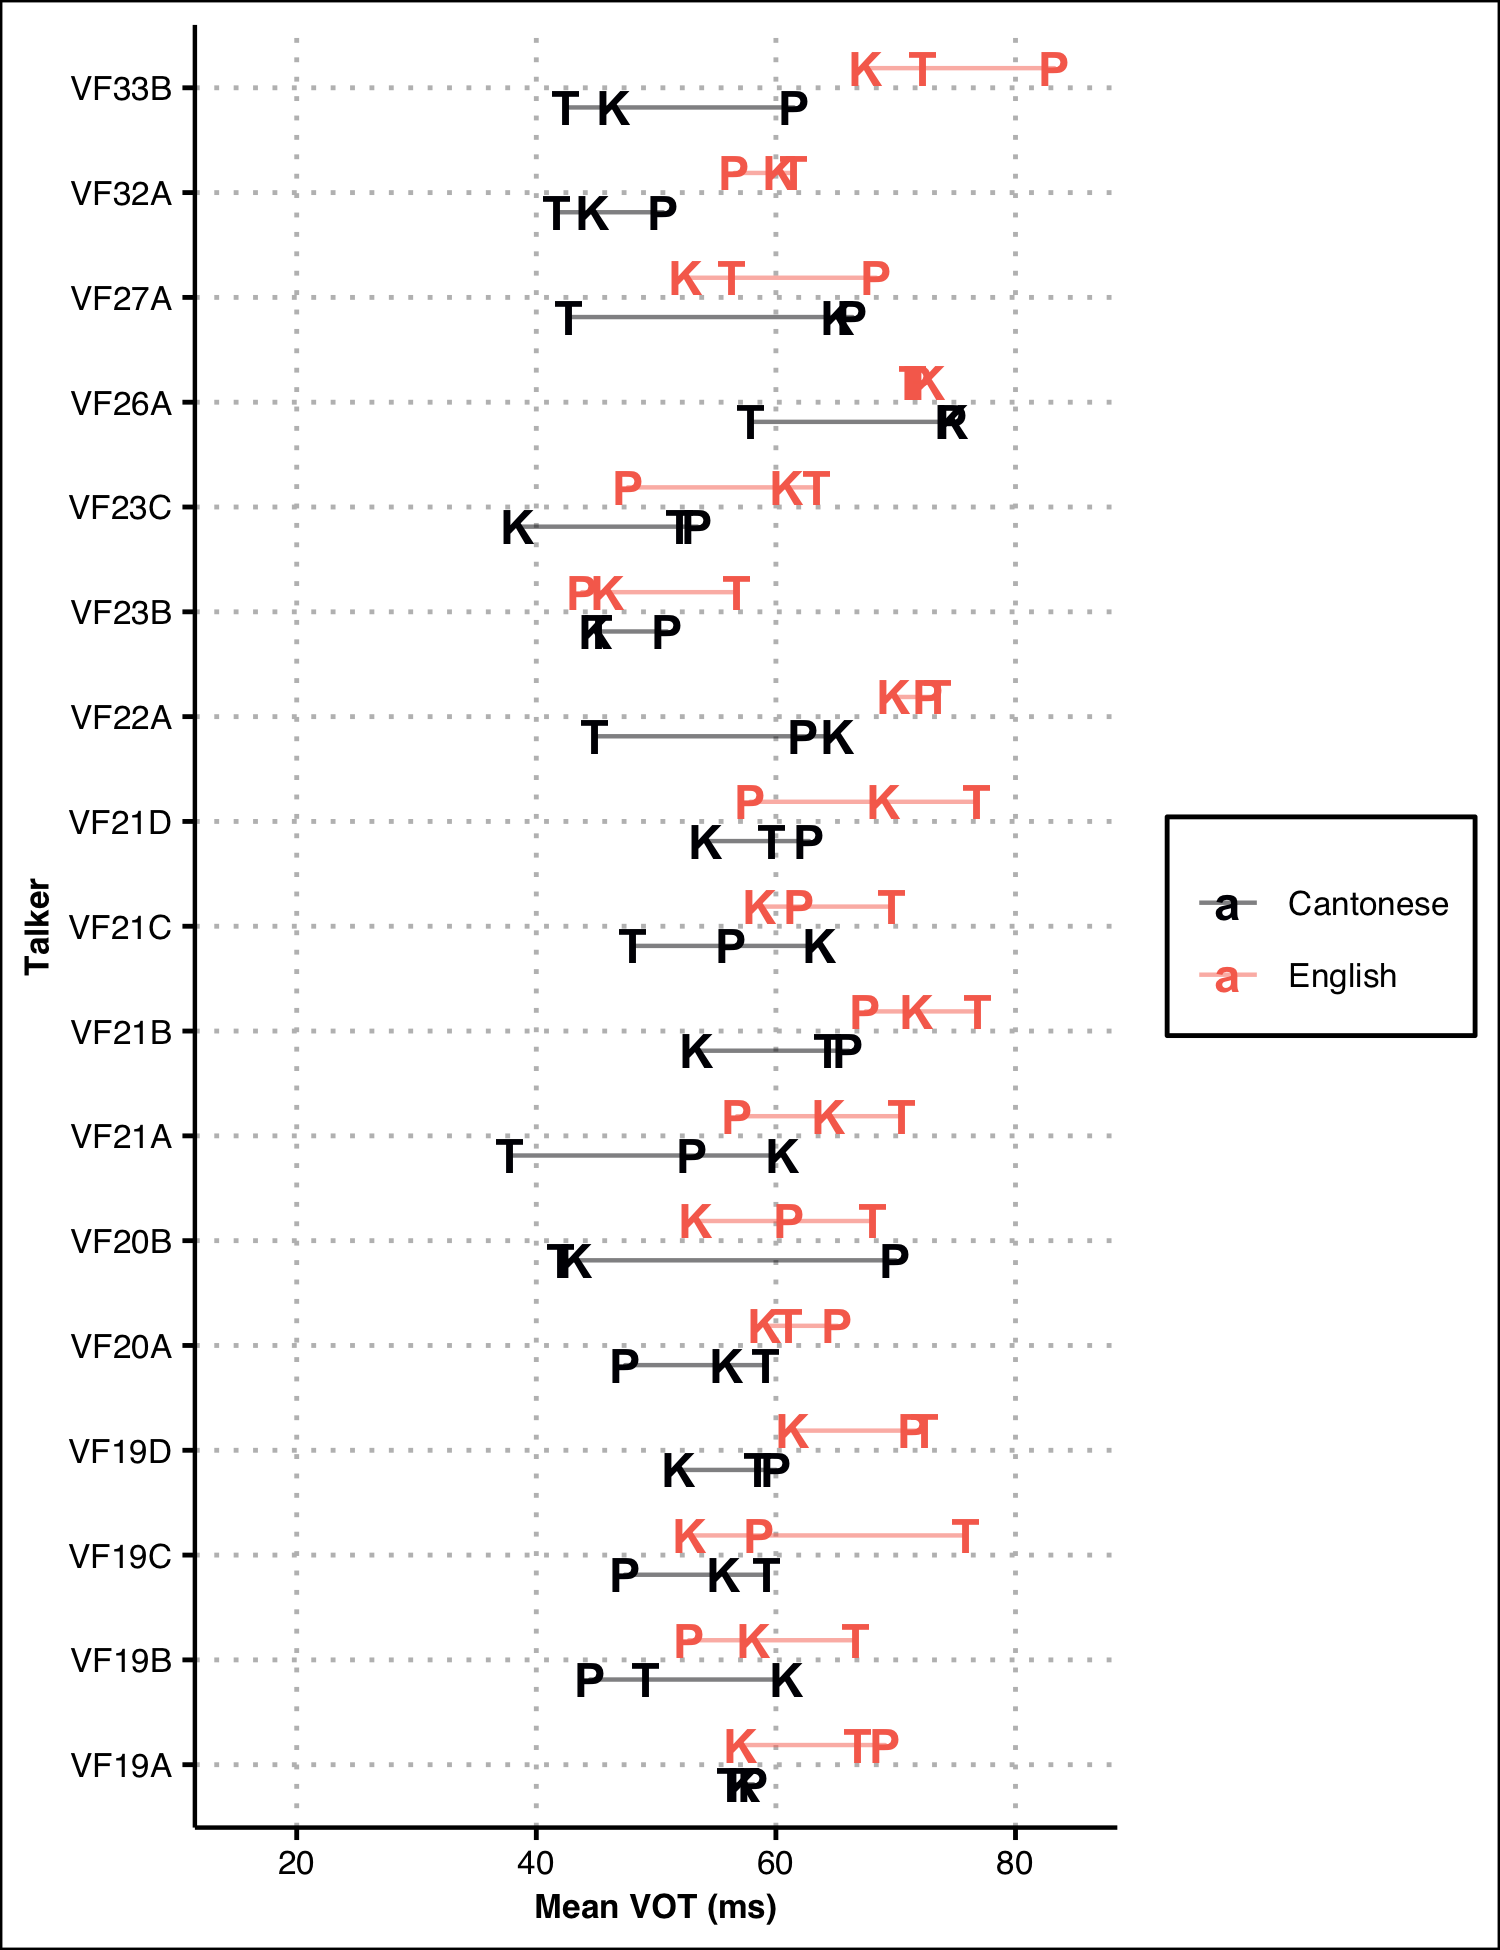
\includegraphics[width=0.9\linewidth]{figures/ch4_ordrel_vf_5in.png} 
  \caption{This figure depicts the ordinal relationships for the female talkers. Each panel depicts the mean VOT and standard error for VOT for each segment, with E(nglish) and C(antonese) in separate rows.}
  \label{ch4:fig:ordrelvf}
  \end{center}
\end{figure}

\begin{figure}[htbp]
  \begin{center}
  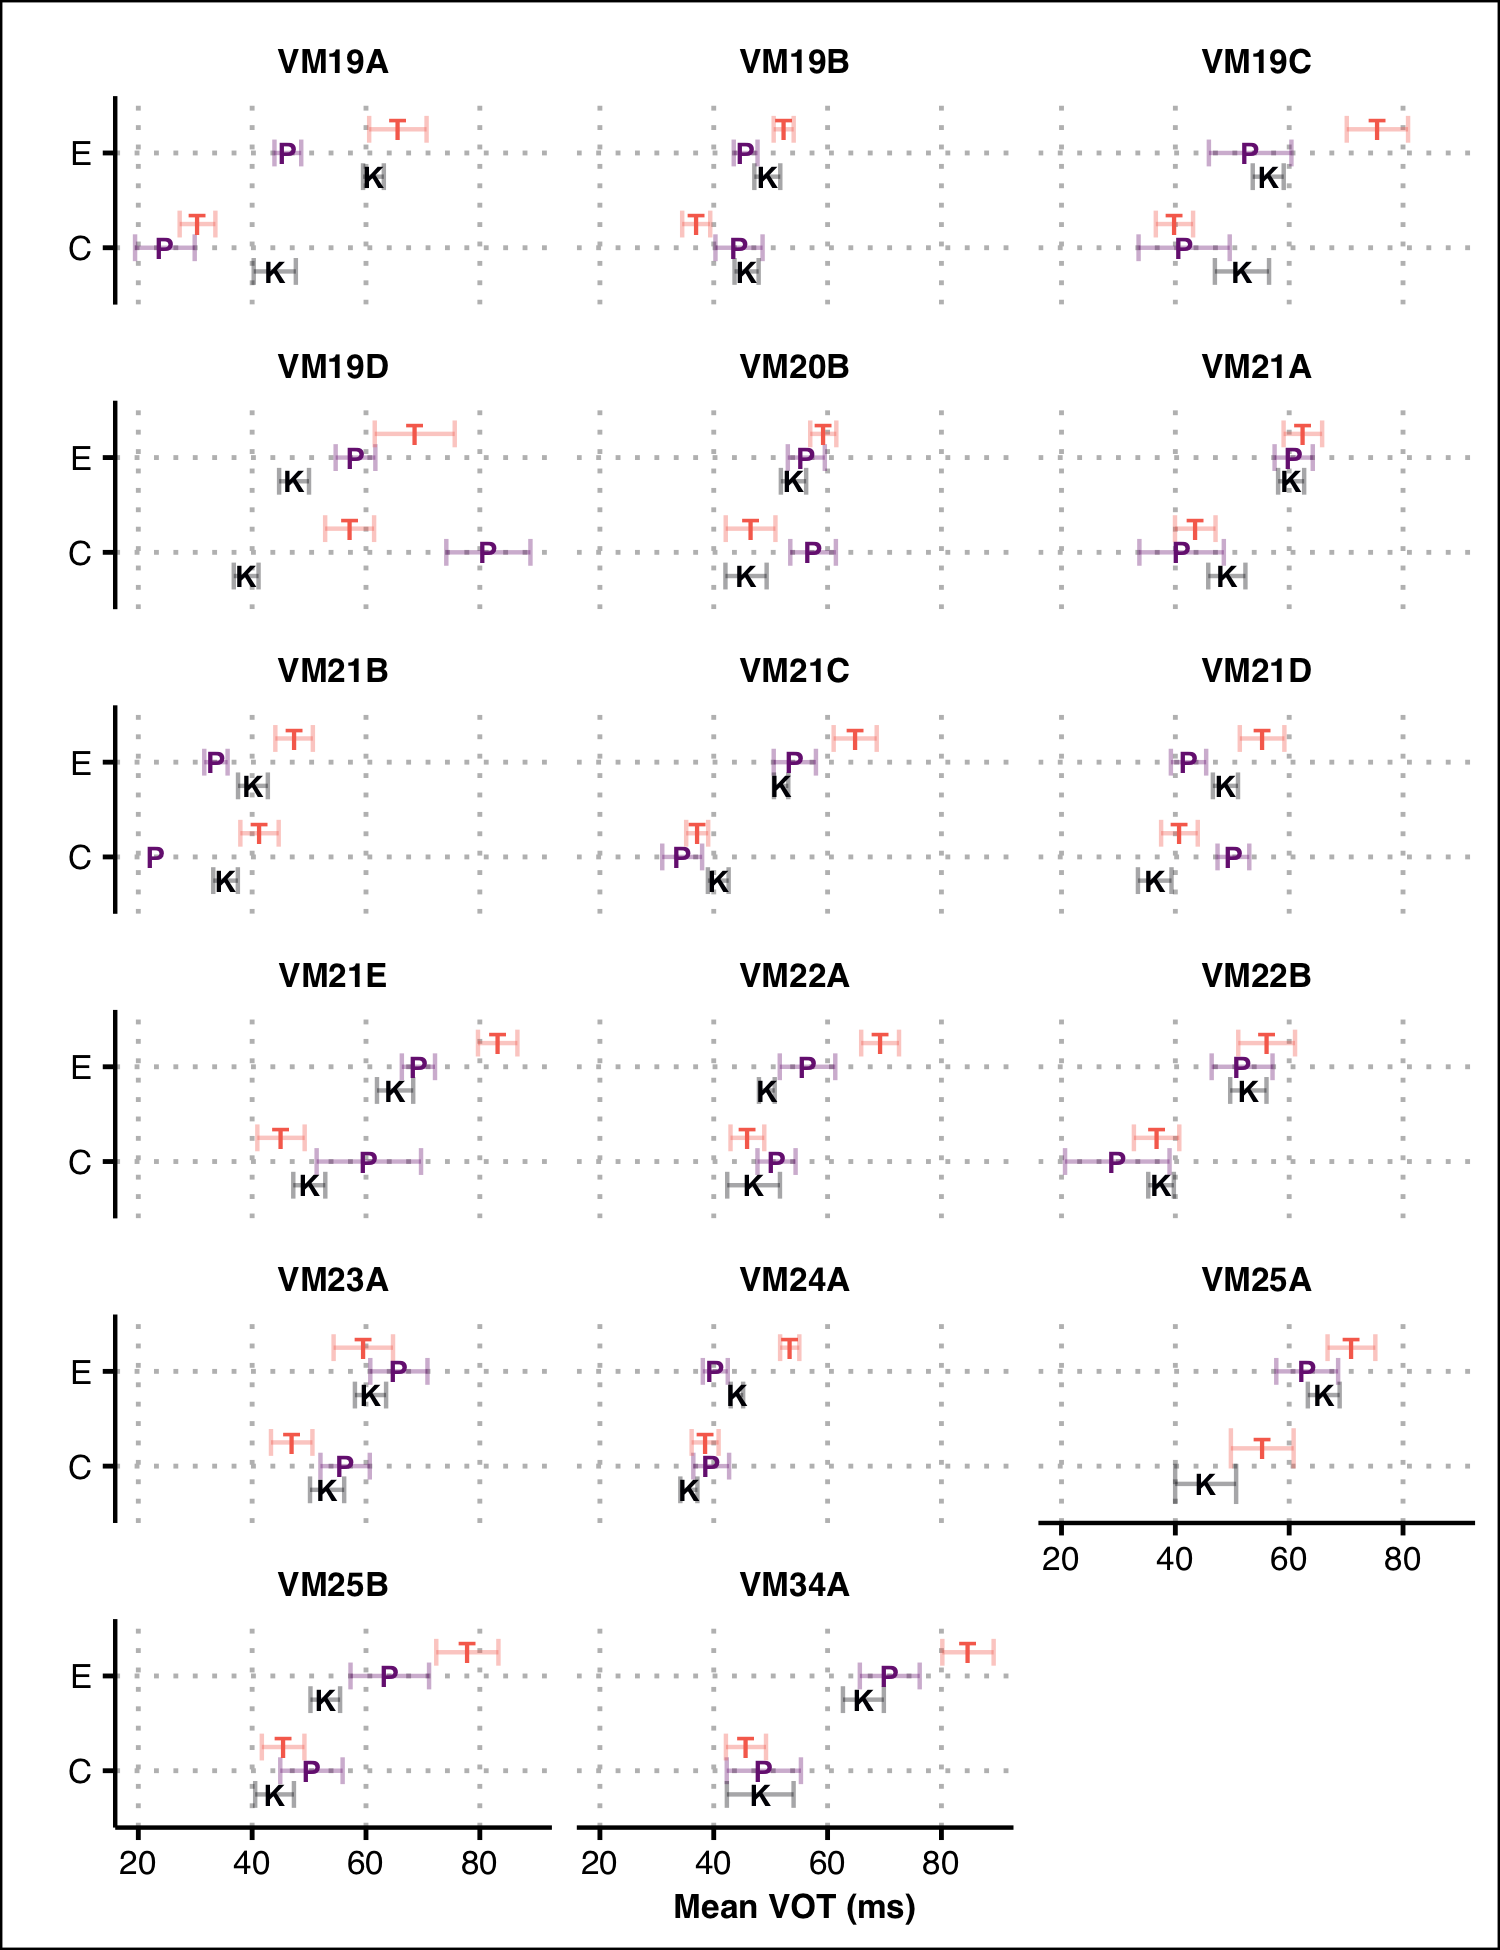
\includegraphics[width=0.9\linewidth]{figures/ch4_ordrel_vm_5in.png} 
  \caption{This figure depicts the ordinal relationships for the male talkers. Each panel depicts the mean VOT and standard error for VOT for each segment, with E(nglish) and C(antonese) in separate rows.}
  \label{ch4:fig:ordrelvm}
  \end{center}
\end{figure}


\subsection{Pairwise correlations}\label{ch4:sec:correlations}
% I personally don’t quite understand enough about your correlation analysis…a failing on my part, but maybe helped through extended discussion, is how sufficient using the residuals is for correcting for speech rate.
% it’s also unclear to me whether the talkers were paired with themselves within the correlations presented in Table 2 (i.e., are these analogous to the Chodroff and Wilson 2017 figures?)
% did you do any correction for significance with 15 correlations?
To examine the relationship between stops within and across languages, 15 pairwise Pearson's \textit{r} correlations were calculated across talker means. Each correlation compares talkers means for two different segments. The full pairwise correlations include three within English, three within Cantonese, and nine comparing English to Cantonese. These correlations are reported along with Holm-adjusted \textit{p}-values to account for multiple comparisons. This analysis uses the \textit{psych} \citep{revelle_2021_psych} package in R \citep{r_2021}. As in \citet{chodroff_2017_structure}, this correlation analysis aims to elucidate within-talker invariance and between-talker variability. While using means ignores information about within-category variability, prior work sets up strong, clear expectations about how the mean values for long-lag VOT pattern \citep{chodroff_2017_structure, cho_1999_vot}. 

Table \ref{ch4:tab:correlations} summarizes the output of all 15 correlations in text form. Figures \ref{ch4:fig:correlations1} and \ref{ch4:fig:correlations2} depict each of the 15 correlations in the fashion of \cite{chodroff_2017_structure}. While there is some evidence for both within- and across-language structured variation, the correlations reported here are considerably lower than prior work on English read speech. Similar within-language comparisons had $r>0.7$ \citep{chodroff_2017_structure, chodroff_2019_l2}. With the exception of the English /p/ $\sim$ /k/ ($r=0.70$, $p<0.001$), all of the correlations were either moderate ($0.5<r<0.7$; $p<0.01$) or not significant. Within-English correlations were the most consistent---all three had \textit{r} at or above 0.65 (p $<$ 0.001). Of the within-Cantonese correlations only /p/ $\sim$ /t/ was significant (\textit{r}$=$ 0.59; \textit{p}$=$0.003), though the correlation for /p/ $\sim$ /k/ was marginal (\textit{r}$=$ 0.44; \textit{p}$=$0.08). Two of three across-language correlations at the same place of articulation were significant, with moderate \textit{r} values (/p/ $\sim$ /p/: \textit{r}$=$0.62, \textit{p}$=$0.001; /k/ $\sim$ /k/: \textit{r}$=$0.57, \textit{p}$=$0.004). Of the across-language comparisons that do not share a place of articulation, only one was significant---Cantonese /k/ $\sim$ English /p/ (\textit{r}$=$0.58, \textit{p}$=$0.003).

\begin{figure}[htbp]
  \begin{center}
  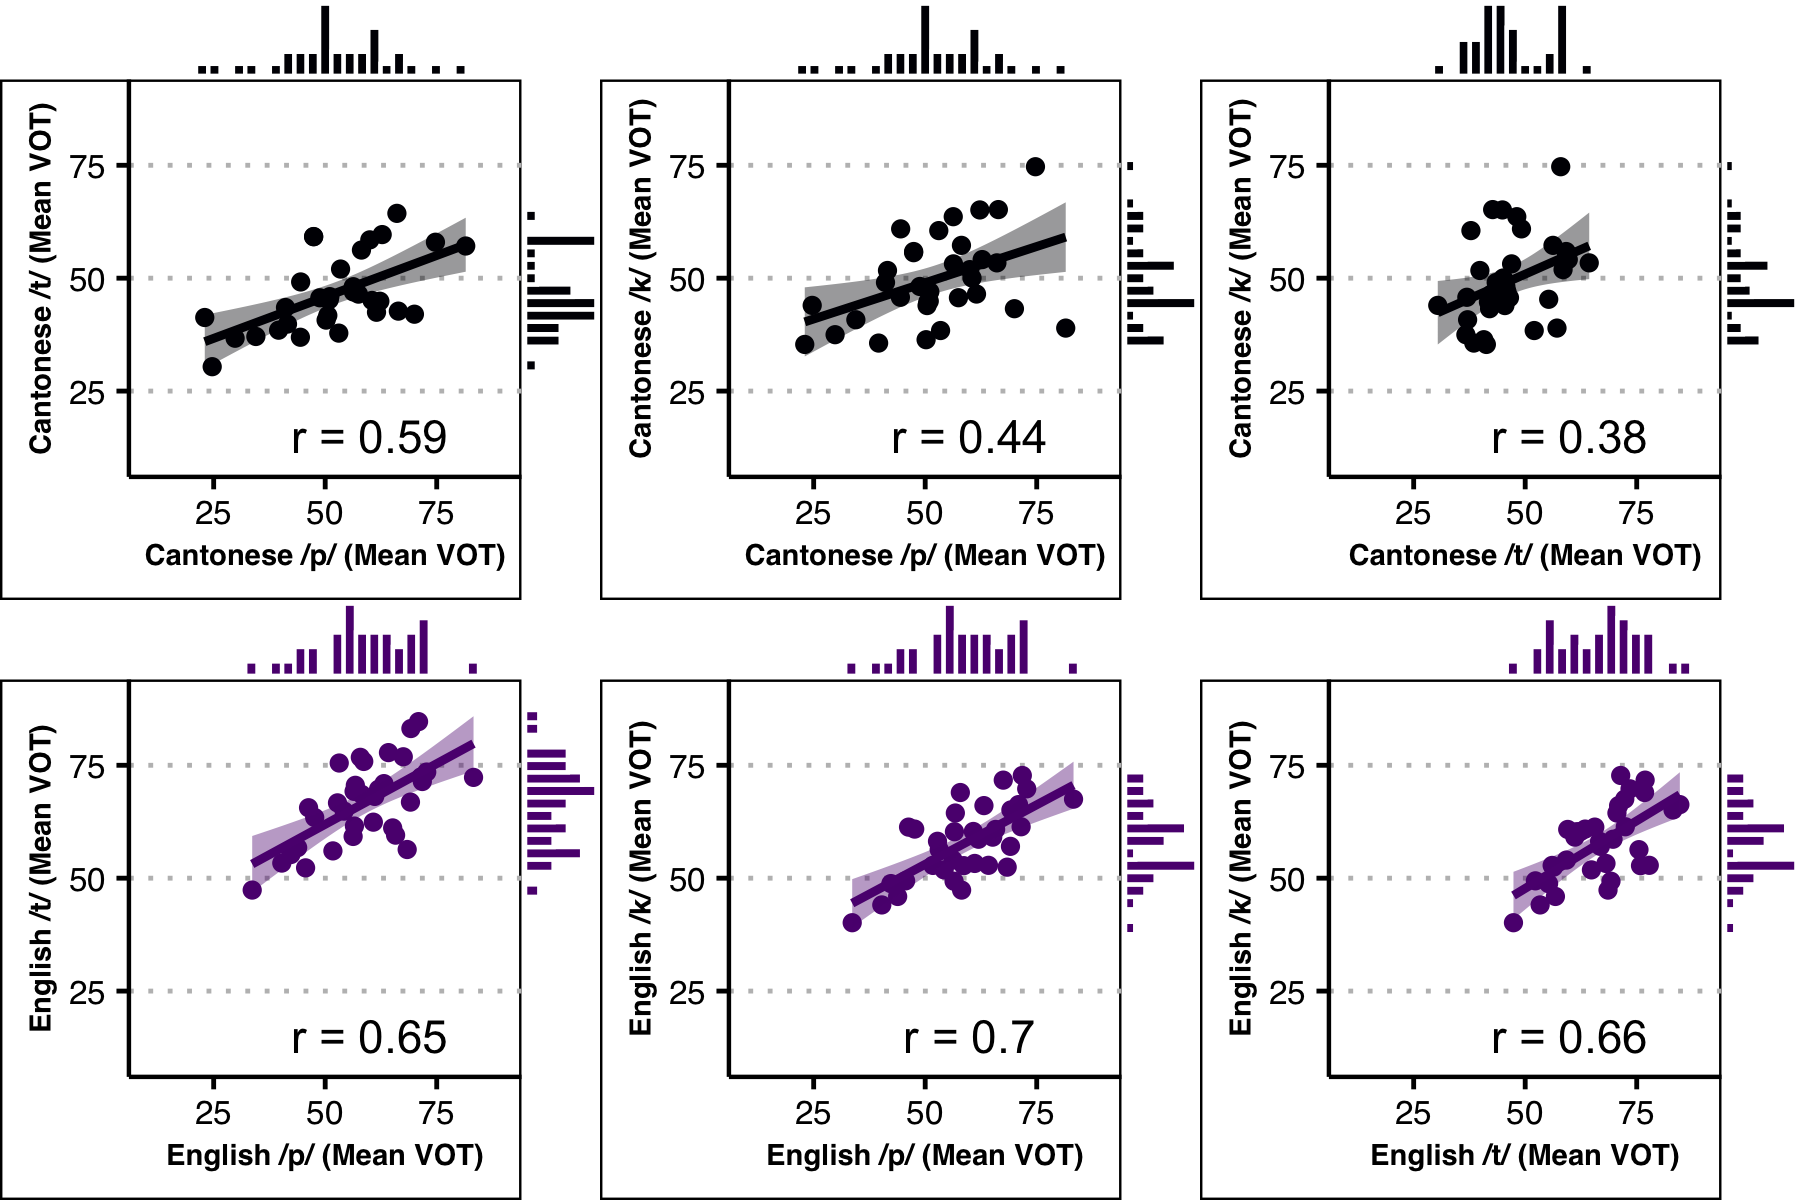
\includegraphics[width=0.9\linewidth]{figures/ch4_correlations1_5in.png} 
  \caption{Correlations!}
  \label{ch4:fig:correlations1}
  \end{center}
\end{figure}

\begin{figure}[htbp]
  \begin{center}
  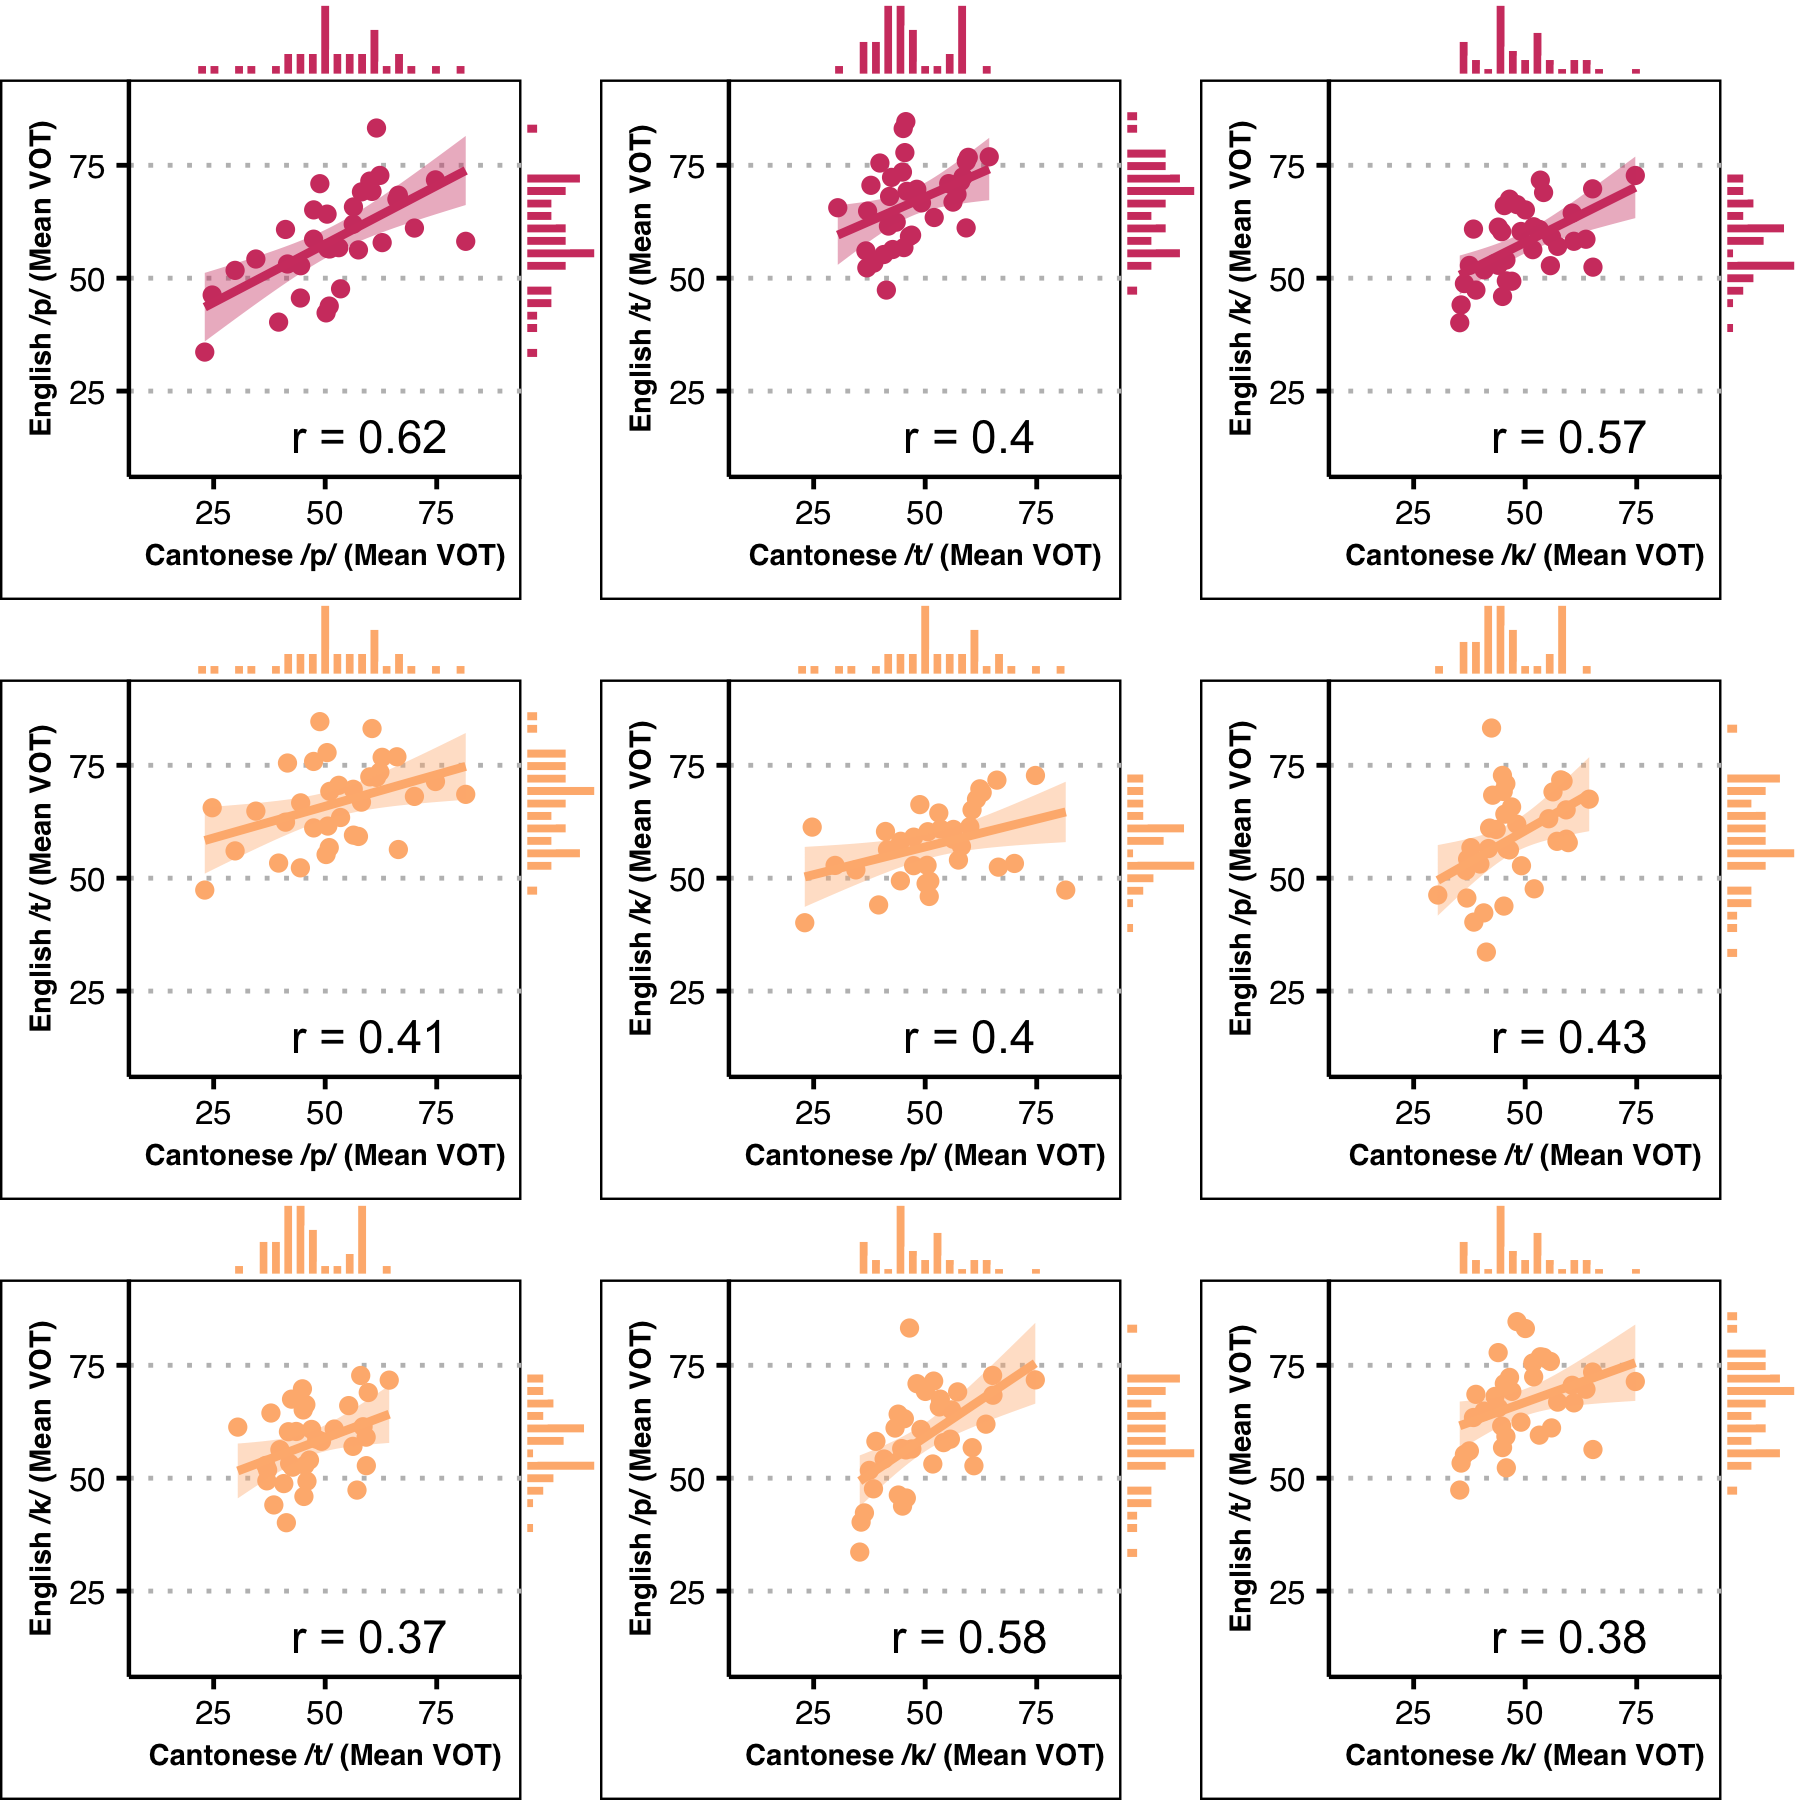
\includegraphics[width=0.9\linewidth]{figures/ch4_correlations2_5in.png} 
  \caption{Correlations!}
  \label{ch4:fig:correlations2}
  \end{center}
\end{figure}

\begin{table}[htbp]
  \caption{All 15 correlations based on raw mean VOT---and separately, VOT residuals after accounting for speaking rate---for each talker, language, and segment. Each row indicates the comparison, Pearson's \textit{r}, and the Holm-adjusted \textit{p}-value given 15 comparisons.}
    \label{ch4:tab:correlations}
    \centering 
    \footnotesize
    \begin{tabular}{ll|ll|ll}
      \toprule
      &   & \multicolumn{2}{l|}{\textbf{Raw}} & \multicolumn{2}{l}{\textbf{Residualized}} \\
      \textbf{Type}     & \textbf{Comparison} & \textit{r}        & \textit{p}       & \textit{r}            & \textit{p}            \\
    \midrule
    Within-Cantonese  & Cantonese /p/ $\sim$ Cantonese /t/    & 0.59    & 0.003       & 0.59   & 0.003    \\
    Within-Cantonese  & Cantonese /p/ $\sim$ Cantonese /k/    & 0.44    & 0.08        & 0.55   & 0.01     \\
    Within-Cantonese  & Cantonese /t/ $\sim$ Cantonese /k/    & 0.38    & 0.11        & 0.34   & 0.21     \\
    \midrule
    Within-English    & English /p/   $\sim$  English /t/     & 0.65    & $<$0.001    & 0.63   & 0.001    \\
    Within-English    & English /p/   $\sim$  English /k/     & 0.70    & $<$0.001    & 0.70   & $<$0.001 \\
    Within-English    & English /t/   $\sim$  English /k/     & 0.66    & $<$0.001    & 0.60   & 0.002    \\
    \midrule
    Across-language   & Cantonese /p/  $\sim$ English /p/     & 0.62    & 0.001       & 0.57   & 0.01    \\
    Across-language   & Cantonese /t/  $\sim$ English /t/     & 0.40    & 0.11        & 0.35   & 0.21    \\
    Across-language   & Cantonese /k/  $\sim$ English /k/     & 0.57    & 0.004       & 0.54   & 0.01    \\
    \midrule
    Across-language   & Cantonese /p/  $\sim$ English /t/     & 0.41    & 0.11        & 0.29   & 0.31    \\
    Across-language   & Cantonese /p/  $\sim$ English /k/     & 0.40    & 0.11        & 0.29   & 0.31    \\
    Across-language   & Cantonese /t/  $\sim$ English /p/     & 0.43    & 0.08        & 0.37   & 0.20    \\
    Across-language   & Cantonese /t/  $\sim$ English /k/     & 0.37    & 0.11        & 0.27   & 0.31    \\
    Across-language   & Cantonese /k/  $\sim$ English /p/     & 0.58    & 0.003       & 0.59   & 0.003   \\
    Across-language   & Cantonese /k/  $\sim$ English /t/     & 0.38    & 0.11        & 0.37   & 0.20    \\
    \bottomrule
    \end{tabular}
\end{table}

\citet{chodroff_2017_structure} also repeat the correlation analysis in a way the coarsely accounts for speaking rate. This consideration is important, as the local speaking rate is known to influence long-lag VOT in spontaneous speech \citep{stuartsmith_2015_private} and because prior work demonstrates both talker and language effects on speech rate \citep{bradlow_2017_rate}. In comparing the two versions of the correlation analysis, \citeauthor{chodroff_2017_structure} found that ``the magnitudes of the correlations among voiceless stops did not deviate from the original magnitudes, demonstrating that differences among talkers in the realization of these sounds cannot be reduced to talker-specific speaking rates'' \citeyearpar[][p. 34]{chodroff_2017_structure}. 

I conducted a similar analysis here, using means calculated over \textit{residual} VOT values from a simple linear regression in which VOT was predicted by average phone duration within the word. Average phone duration is a proxy for speech rate. It was calculated as the difference between the word's AutoVOT-estimated onset and force-aligned offset, divided by the number of segments in the canonical form of the word. The results---Pearson's \textit{r} and Holm-adjusted \textit{p} values---are reported in the rightmost columns of Table \ref{ch4:tab:correlations}. Qualitatively, the results mostly mirror the correlations based on raw VOT, though there are some differences in significance and magnitude. This difference can likely be attributed to the generally weak correlations found. 

While these relationships indicate some degree of articulatory reuse, the overall picture is far from compelling, particularly when considered alongside the results of the analysis of the ordinal relationships in Section \ref{ch4:sec:ordrel}. Compared to prior work, these correlations are less consistent and generally weaker.

The next steps in \citeauthor{chodroff_2017_structure}'s \citeyearpar{chodroff_2017_structure} methods focus on validating the strength of the correlations. Their approach includes estimating confidence intervals for the correlations using a bootstrap procedure \citep{chodroff_2017_structure}. In a later paper, they simulate what would emerge from a purely ordinal relationship between stops and demonstrate that the observed correlations are much stronger—ultimately arguing for a uniformity constraint on phonetic variation \citep{chodroff_2019_covariation}. Given that the correlations found in this chapter are drastically lower and largely do not adhere to the expected ordinal relationships, the remainder of this analysis takes a different approach.

\subsection{Linear mixed effect model}\label{ch4:sec:lmem}

The analysis in the section leverages a Bayesian multilevel linear model to elucidate the sources of variation within and across talkers. As Bayesian modeling emphasizes the estimation of effect magnitudes, the model can be used to assess how talker's sound categories compare to one another while simultaneously accounting for factors known to influence long-lag VOT. This modeling approach is more in line with the generative modeling approach advocated for by \citet{haines_2020_theoretically}---in a way that the correlation and ordinal relationships analyses in the preceding sections are not. This section proceeds as follows. Section \ref{ch4:sec:bayesianinference} describes Bayesian modeling and inference in broad terms and points the reader towards sources for further reading. Section \ref{ch4:sec:model} motivates and describes the structure of the model used in this chapter. Lastly, Section \ref{ch4:sec:results} reports the results of the model. All code used in this analysis is available at \hl{a GitHub repository that will be made public later on}.

\subsubsection{Bayesian inference}\label{ch4:sec:bayesianinference}
The corpus sample was analyzed with a Bayesian multilevel linear model using the brms package in R \citep{burkner_2017_brms,r_2021}. The brms package provides a simple, formula-based interface to Stan---a widely used probabilistic programming language for estimating Bayesian statistical models \citep{stan_2021}. Bayesian models are desirable in the case of modeling multilingual VOT for both practical and theoretical reasons. Practically, they are not subject to the convergence problems that plague complex frequentist models. Theoretically, they allow for graded statements regarding the strength of evidence for all parameters, both population level (i.e., fixed effects) and group level (i.e., random effects) parameters. While there are many other benefits, readers are referred to \citeauthor{vasishth_2018_bayesian}'s \citeyearpar{vasishth_2018_bayesian} recent in-depth tutorial paper on Bayesian modeling in the phonetic sciences for further argumentation. 

Inference in Bayesian models is based on the posterior distributions of parameters in the model, which reflect the range and probability of credible values for parameters. The posterior combines information from prior knowledge and the likelihood of observing the data given the specified model. While some Bayesian models use detailed and specific prior knowledge, it is perhaps more common to use weakly informative, regularizing priors \citep{gelman_2017_prior}, which constrain the parameter space to possible values and down weight extreme or unlikely values. The model described in the next section uses regularizing priors. 

In line with how Bayesian models emphasize parameter estimation in a probabilistic framework, it is also possible to compare parameters. \citet{gelman_2012_multiple} argues that because of the rich probabilistic information in each parameter's posterior distribution, making multiple comparisons within the model is not problematic, as it is in the case of frequentist statistics. Further, while parameter estimation remains the focus, there are decision criteria that facilitate determining whether the difference between two parameters is important or not. One such technique is to use \citeauthor{kruschke_2011_rope}'s \citeyearpar{kruschke_2011_rope} ROPE+HDI method. The ROPE is a ``region of practical equivalence'' surrounding the null value. The HDI is the highest density interval typically used to describe Bayesian posterior distributions. \citeauthor{kruschke_2011_rope}'s \citeyearpar{kruschke_2011_rope} decision criterion is simple: if the HDI falls entirely within the ROPE, then the null value can be accepted; if the HDI falls entirely outside the ROPE, then it can be rejected; if there is overlap, then a decision should be withheld. In the case of standardized data, \citet{kruschke_2011_rope} recommends the convention of setting a ROPE to be [$-$0.1, 0.1]---half the size of a small Cohen's \textit{d} effect. While Bayesians tend to shy away from using decision criteria, it nonetheless provides a useful scaffolding for interpreting the magnitudes of standardized effects, when presented alongside the full posterior distributions. 

\subsubsection{Modeling multilingual VOT}\label{ch4:sec:model}

VOT was modeled with a multilevel linear model using the formula in \ref{ch4:num:formula}. While this does not represent the maximal model \citep{barr_2013_maximal}, it instead follows guidelines for parsimonious model building \citep{bates_2018_parsimonious}, in which the parameters of direct interest are included as random slopes, and the controlling parameters are not.

\begin{equation}\label{ch4:num:formula}
  \text{VOT} \sim 0 + \text{Phone} + \text{APD} + (0 + \text{Phone} + \text{APD }|\text{ Talker}) + (1 | \text{Pause}) + (1 | \text{Word})
\end{equation}


% The interpretation of the linear ME model needs to be fleshed out and related more clearly to your original research question(s)
% Frame this section as being motivated by the lack of strong uniformity, and by Chodroff's analysis of the random effects structure
% To better account for variation due to known factors such as speech rate and the presence of a preceding pause, a linear mixed-effects model was fit with the \textit{lme4} package \citep{bates_2015_lme4} in R \citep{r_2021}. The model's aims were two-fold: estimating the effect of language by segment and elucidating the sources of variation in the random effects structure. Analyzing the data in this way mitigates the issues with conducting statistical tests on talker means, which ignores much of the variation in the data \citep{haines_2020_theoretically}. 

One of the main benefits of multilevel modeling is partial pooling, where information for different levels of a variable is shared across those levels. \citeauthor{mcelreath_2020_sr} argues that ``any batch of parameters with exchangeable index values can and probably should be pooled [where exchangeable] just means the index values have no true ordering'' \citeyearpar[][p. 435]{mcelreath_2020_sr}. Pooling can be done for both intercepts and slopes, much in the way that frequentist models allow for slopes and intercepts to vary in the random effects structure. 

Details about how the parameters were specified are as follows.  

\begin{description}
  \item[VOT] was the dependent variable---it was standardized, in order to facilite prior and ROPE specification. 
  \item[Phone] encodes both place of articulation and language, such that there are six levels---one for each phone in each language. Phone uses index variable coding, as advocated for by \citet{mcelreath_2020_sr}. This means that the model estimates a separate intercept for each of the phones, but not an overall intercept. Ultimately, this facilitates the comparisons of interest.  
  \item[Average Phone Duration, ``APD'',] represents the average duration of phones within the word. It was calculated as the difference between the word's AutoVOT-estimated onset and the force-aligned word offset, divided by the number of segments in the canonical form of the word. As noted earlier, average phone duration serves as a proxy for local speaking rate. A word-internal measure is desirable, as many tokens were preceded by a pause and thus lack the preceding context from which to calculate it. Average phone duration was also standardized. 
  \item[(Preceding) Pause] indicates whether or not the token occurred after a pause or not. Pauses were defined as X. Preceding pause was treated as a grouping parameter.
  \item[Word] ... 
\end{description}

% The interaction for Language $\times$ Place was included in the model---it directly addresses the research question relating to whether or not bilinguals maintain a difference across languages for these sounds. As apparent in the above list, the categorical fixed effects all employed weighted effect coding, using the \textit{wec} R package \citep{nieuwenhuis_2017_weighted}. This decision follows \citet{chodroff_2017_structure} and facilitates the interpretation of the simple effects in light of the interaction term \citep{brehm_2021_contrasts}. Additionally, random intercepts for Talker and Word were included, as were by-Talker slopes for Language, Place, and their interaction. While this does not represent the maximal model \citep{barr_2013_maximal}, it instead follows guidelines for parsimonious model building \citep{bates_2018_parsimonious}, in which the parameters of direct interest are included as random slopes, and the controlling parameters are not.


\subsubsection{Results}\label{ch4:sec:results}




% Add full table of LME results and some data viz

% At an $\alpha=0.01$ threshold, the model returned a significant intercept ($\beta=0.18$, $SE=0.49$, $p<0.001$), significant main effects for Average Phone Duration ($\beta=0.32$, $SE=0.01$, $p<0.001$) and Preceding Pause (True; $\beta=0.12$, $SE=0.02$, $p<0.001$), as well as significant simple effect for Language (English; $\beta=0.15$, $SE=0.03$, $p<0.001$), indicating that VOT was longer at slower speech rates, after pauses, and in English, compared to the weighted mean. Neither Place nor its interaction with Language was significant. As one of the linear mixed-effects model goals was to assess the effect of Language across places of articulation, pairwise post-hoc comparisons were computed for Language $\times$ Place using the \textit{emmeans} package \citep{lenth_2021_emmeans}, with a confidence level of 0.95, and the Kenward-Roger degrees-of-freedom method. The contrast between languages was significant for /t/ ($\beta=-0.38$, $SE=0.09$, $p<0.001$) and /k/ ($\beta=-0.53$, $SE=0.10$, $p<0.001$), but not for /p/ ($\beta=-0.09$, $SE=0.11$, $p=0.39$): VOT is consistently longer in English for /t/ and /k/.

% The second goal of the mixed-effects analysis was to gain insight into the sources of variation through the random effects structure. Of the random effects, the intercepts for Word ($SD=0.20$) and Talker ($SD=0.06$) accounted for the most variation, followed by the by-Talker slope standard deviations for Language ($SD=0.005$), Place T ($SD=0.01$), Place T $\times$ Language ($SD=0.005$), Place K ($SD=0.004$) and Place K $\times$ Language ($SD=0.002$). Talkers and words differ substantially in mean VOT, while the slopes for Place and Language effects appear more consistent across talkers.





\section{Discussion}
% ADD:
% - Limitation of whether the difference between languages is a clear diff, or motivated by timing differences, e.g. Bradlow's speech rate paper as a potential avenue to disambiguate this -> both language and talker-indexical info there

This paper reports a study of long-lag stops in Cantonese-English bilingual speech from the SpiCE corpus described in Chapter \ref{ch:Corpus}. It uses the uniformity framework to assess VOT similarity within and across languages. In broad strokes, the evidence for uniformity both within and across languages was limited. The correlation analysis provides evidence for within-language uniformity and some across-language structure. The magnitudes were largely weak and moderate. These results are corroborated by the random effects structure of the linear mixed-effects model, as more of the variation is attributable to Talker intercepts than to the Language and Place slope effects. In this sense, while there is some degree of structure in VOT variation, it seems weaker than the relationships described in prior work, where strong and clear within-language patterns were observed \citep{chodroff_2017_structure, chodroff_2019_l2}.

The far more interesting outcomes here relate to unexpected results. The ordinal relationships should be interpreted with a grain of salt, as there are several potential explanations not immediately relevant to the research question. For example, means were based on fewer tokens than in prior work (especially for /p/), which may render those proportions less reliable; and, the speech in SpiCE differs in style (conversational vs. read). This outcome is perhaps not surprising, as \citet{chodroff_2017_structure} reported magnitude differences between isolated citation form and connected read speech. Lastly, the error often overlaps in Figure XX, potentially making the ordinal relationships less reliable or meaningful. Another unexpected outcome is that English VOT seems to be consistently longer than in Cantonese---the opposite of what prior work suggested \citep{clumeck_1981_cantonese, lisker_1964_vot}. No explanation is offered here other than to reiterate the casual speech style under examination. Additionally, lab and corpus results often differ \citep{gahl_2012_reduce,chodroff_2017_structure}, as do corpus studies of monolingual and bilingual speech \cite{johnson_2019_probabilistic}. 

While the results here do not necessarily provide evidence for a bilingual crosslinguistic uniformity constraint, they offer insight into what makes bilingual speech unique and provide an empirical description of bilingual long-lag stops. In terms of describing the relationship between the long-lag stops in each language, talkers maintain a crosslinguistic contrast despite stops' proximity---for many talkers---in the long-lag space. The contrast is a strong candidate for a composite category in SLM-r \citep{flege_2021_slmr} and merits further investigation.

% Flesh out this paragraph a bit more, but save something for the general discussion -->
A lack of strong crosslinguistic uniformity has implications for speech perception. Tracking a uniformity-like pattern has been proposed as a mechanism for rapidly adapting to speech across languages \citep{reinisch_2013_retune} and in multilingual talker identification \cite{orena_2019_identifying}. If the results of this study stand, then such a perceptual strategy may have limited use in real communicative contexts, whether or not listeners use it in a lab setting. Overall, this study highlights the need to study spontaneous speech and offers a first pass at leveraging the methods of the uniformity framework to better understand crosslinguistic similarity.

\endinput % -------------------------------------------------------- %

% THE GRAVEYARD OF WORDS


% Define representation, phonetic categories, and exemplar-y model, what it means for categories to be linked, i.e., the composite category of SLM-r

% A consequence of bilingualism is that individuals must navigate overlapping segment inventories. This paper is concerned with what languages share, if anything, in the mental representation of speech sound categories. As representation means different things across linguistic disciplines, defining and situating the term is first necessary. The approach in this chapter largely falls out of the revised Speech Learning Model \citep[SLM-r;][]{flege_2021_slmr} and its exemplar-flavored take on what phonetic categories look like in linguistic systems with more than one language. 

% SLM-r is a widely used and respected model used in second language acquisition and multilingualism research. Unlike some other models in the same space, SLM-r grapples with both perception and production. SLM-r assumes that speech sound categories from different languages exist in a shared phonetic space and are subject to constraints from the perceptual and productive systems. Effectively, don't get too close to each other in perception, and don't get too complicated in production \citep{guion_2003_systems, lindblom_1988_universals, flege_1995_slm}. These constraints lead SLM-r to posit that proximity leads to instability, even if what counts as close remains unclear. Considering how bilinguals are fully capable of maintaining subtle distinctions for similar sound categories across languages \citep[e.g.,][]{sundara_2006_production}, this is not a trivial point to make. 

% So, what does representation look like in this system? SLM-r outlines a few potential outcomes for sound categories in a shared system—they can assimilate or dissimilate. A relatively simple take on this is that assimilation equals shared mental representation, while dissimilation equals separate. The picture is complicated, however, by the idea of imperfect assimilation and what \citeauthor{flege_2021_slmr} term \textit{composite categories}. In the SLM-r, if sounds from two languages are phonetically too close to each other, they will remain linked in a composite category "defined by the statistical regularities present in the combined distributions of the perceptually linked...sounds." \citep[][p. 41]{flege_2021_slmr}. This scenario might be characterized as an imperfectly shared representation, where certain dimensions are kept apart, and others overlap. This particular characterization is salient in a recent meta-analysis of crosslinguistic influence for Spanish and English initial stop consonants. In this study, \citet{casillas_2021_interlingual} found that early bilinguals did not produce ``compromise'' stop categories. That is, early Spanish-English bilinguals did not produce voice onset time that was somehow intermediate to canonical productions by monolinguals of either language. This finding echoes arguments made by \citet{bullock_2009_sociophonetics} on the sophistication and control that bilingual exert over their possible forms. There is no compromise but rather a wide range of forms that bilinguals can deploy according to context.

% % Need to fix a lot in here because Casillas paper really goes against the idea of composite or "compromise" categories

% This idea of composite categories is similar to other concepts in multilingualism literature, namely that of linked categories. While the idea is pervasive, it is somewhat vaguely defined. In a handbook chapter on bilingual phonetics and phonology, \citet{simonet_2016_bilingualism} describes ``links or connections of one sort or another between the phonetic categories'' (p. 10). \citeauthor{simonet_2016_bilingualism} then notes that ``these connections...are transiently strengthened in contexts that induce the activation of both languages and inhibited in contexts that favor the use of only one of the languages'' \citeyearpar[][p. 10]{simonet_2016_bilingualism}. Presumably, sound categories could be linked whether they surface in dissimilated or composite (assimilated) forms. The idea behind composite categories is more fully fleshed out and theoretically useful than mere links in grappling with how representation works in the bilingual mind. 

% Most prior work in crosslinguistic influence has focused on sounds that are phonologically similar yet phonetically distinct. A common example of this arises from languages that differ in their initial stop voicing contrasts. North American English contrasts long- and short-lag stops in initial position. Conversely, Spanish (among many languages) contrasts short-lag and prevoiced initial stops. As will become apparent later in the introduction, there is strong evidence for a crosslinguistic link between English long-lag and Spanish short-lag stops, despite the clear difference in voice onset time. The relative position of these sounds within each language can account for why they are linked together; in each case, the linked sound occupies the position closest to long-lag, on a spectrum ranging from long-lag to short-lag to prevoiced. The primacy of ``relative phonetics'' was put forth in \citeauthor{chang_2015_similarity}'s \citeyearpar{chang_2015_similarity} chapter on similarity in bilingual phonetics and phonology. \citeauthor{chang_2015_similarity} argues that crosslinguistic influence at the segmental level tends to occur between sounds that share ``(1) similar positions in the respective phonemic inventories (when considering the contrastive feature oppositions---or, more broadly, the `relative phonetics'---of the sounds in relation to other sounds in the inventory), and (2) similar distributional facts'' \citeyearpar[][p. 201]{chang_2015_similarity}. This approach to similarity emphasizes a general role for abstraction but does not necessarily invite a formal phonological analysis. In a similar vein, \citeauthor{flege_2021_slmr} argue that similarity ``must be assessed perceptually rather than acoustically because acoustic measures sometimes diverge from what listeners perceive'' \citeyearpar[][p. 33]{flege_2021_slmr}. At this point, ``relative phonetic'' and perceptual similarity seem to be a prerequisite for considering a link between two sound categories and can be used to account for when and where crosslinguistic influence occurs. It does not outline what happens after sounds are ostensibly linked to one another nor opine on the nature of representation for the sound categories in question. 

% \citeauthor{flege_2021_slmr} make a clear appeal to phonetic similarity for assessing assimilation. This appeal is evident in how it steps back from making phonological arguments in general and in its exemplar-flavored account. The SLM-r posits that sound categories ``are defined by the statistical properties of input distributions'' \citeyearpar[][p. 40]{flege_2021_slmr}. In the case of assimilation, there is a single distribution for both languages---a shared representation. Composite categories are considered a special type of assimilation in the SLM-r, though given the results of \citeauthor{casillas_2021_interlingual}'s \citeyear{casillas_2021_interlingual} meta-analysis, they may not be an appropriate characterization of early bilinguals' systems. In the case of dissimilation, the sound categories move apart and comprise separate distributions---separate representations. While \citeauthor{flege_2021_slmr} argue that crosslinguistic influence provides a diagnostic to test for the presence or absence of dissimilation, but also state that ``A method did not exist in 1995 for determining when a new L2 phonetic category had been formed and, alas, the same holds true today'' \citeyearpar[][p. 41]{flege_2021_slmr}. It can be surmised from this that crosslinguistic influence is not a perfect diagnostic. 

% % the flow is off in this part

% In any case, the focus on distributions of experienced exemplars fits in well with the psycholinguistics literature that argues for the primacy of position-specific allophones \citep{mitterer_2018_allophones}, against the use of phonological features in accounting for speech behavior \citep{llompart_2018_acoustic}, and against equating theoretical categories with mental categories more broadly \citep{samuel_2020_resist}.

% The theoretical framework adopted here leans much harder into the phonetics side of the equation and takes exemplar-style sound categories for position-specific allophones as the level of abstraction. The specific categories considered in this chapter are likely subject to some form of assimilation. One of the questions taken up in this chapter is whether this assimilation is complete or takes the form of a composite category. In all cases, crosslinguistic influence---phonetic similarity or dissimiarily---for linked sounds is measured by comparing distributions of measurements, typically in the context of null hypothesis significance testing. The following paragraphs provide a review of the literature on crosslinguistic influence for stop consonants. 


% %Phonetic similarity is typically assessed by distilling either the entire signal () or a subset of relevant acoustic dimensions () and measuring the distance between relevant categories (e.g., Euclidean distance). Applying phonetic versions of similarity to bilingualism is straightforward, though it assumes that the measures used are appropriate in both languages. On the other hand, phonological similarity is typically assessed through distributional () or feature-based mechanisms (). Translating these phonological metrics to a bilingual system, however, is complicated. It requires making a multitude of assumptions about the nature of each language's inventory and ensuring some form of shared currency (i.e., a feature set). 

% % Define phonological similarity, and phonetic similarity, and what it means to be phonologically similar, but arise from a different part of the mental space, again i think exemplars and composite categories are the way to go here


% \hl{intro drafted up to here}

% More in depth review of CLI work -->
% One example is the comparison between initial voiceless stops in English (long-lag) and Spanish (short-lag). Despite the substantial phonetic differences, these sounds are clearly linked in the bilingual mind \citep{fricke_2016_phonetic, antoniou_2010_context, goldrick_2014_switching, sundara_2006_production}. 

% The following studies focus on telling initial stops apart when the stops under consideration are short-lag and long-lag stops, respectively. In most cases, the difference in voice onset time arises because the languages considered are English and a language with a different initial voicing contrast, as with the example given earlier in this chapter. 

% \hl{summary of lab CLI here} \citep{fricke_2016_phonetic, antoniou_2010_context, goldrick_2014_switching, sundara_2006_production}. % add more!

% These studies demonstrate phonetic convergence---or assimilation---in two ways. First, VOT is shorter for English initial stops produced by bilinguals when compared to monolingual control groups. This result is attributed to the influence on English long-lag stops from the short-lag category in the other language. Second, bilinguals appear more likely to produce lead voicing in initial English voiced stops compared to English monolinguals \citep{sundara_2006_production}. In both cases, evidence of crosslinguistic influence arises from comparing bilinguals to monolinguals. Corpus research demonstrates that Spanish-English bilinguals produce shorter, more Spanish-like VOT in the lead up to an English-to-Spanish code switch \citep{fricke_2016_phonetic, bullock_2009_sociophonetics}. 

% The studies mentioned so far focus on VOT, but represent a small subset of the crosslinguistic influence literature. There are many examples of contrasts that are maintained across languages, yet still subject to crosslinguistic influence---for example, with vowels \citep{guion_2003_systems}, laterals \citep{amengual_2018_laterals,barlow_2014_aoa}, and fricatives \citep{peng_1993_influence}). % flesh this paragraph out, and describing how the work on other speech sound is relevant to the quesitons here, noting that in some cases the choice of acoustic measures is more challenging 

% The ability to examine crosslinguistic influence between phonetically and/or phonologically similar sounds hinges on the presence of an observable difference under some set of conditions. This observable difference could take any number of forms---acoustic, gestural, or cognitive (i.e., retrieval time). The sounds typically selected are not discussed as being the same---phonetic character choice notwithstanding. As such, links tend to be described as connecting similar and subject-to-influence sounds that ultimately have distinct representations in either the phonetics, the phonology, or both \citep{antoniou_2010_context,simonet_2016_bilingualism,bullock_2009_sociophonetics}. In the revised Speech Learning Model (SLM-r) \citep{flege_2021_slmr} introduced earlier, these examples would be considered composite categories---combined distributions of phonetic information from linked categories that presumably retain ``peaks'' for each language. While composite categories are widely attested, there are fewer good examples of full category convergence, at least in the early bilingualism literature. One example comes from a lab-based study of Mandarin-English bilingual children in which highly proficient 5--6 year olds did not differ in VOT across Mandarin and English long-lag stops, despite differences across the monolingual comparison groups \citep{yang_2019_vot}. This suggests that the difference is either too small to maintain or that 5--6 year old children have not yet mastered it. The claims in \citep{yang_2019_vot} should be tempered, however, as language mode was not well-controlled for and adult bilingual behavior was not considered. % Describe more examples of full convergenge.

% Despite some inroads, there is nonetheless a distinct paucity of work examining highly phonetically similar speech sounds across languages, even when such a connection would make sense. A recent study of crosslinguistic influence in Cantonese-English bilinguals compares English long-lag and Cantonese short-lag stops in the context of a language switching paradigm \citep{tsui_2019_switching}. While this comparison clearly reflects the need for stimuli to be acoustically distinct beforehand, it glosses over the fact that both languages contrast short-lag and long-lag VOT in initial position. The best candidates for linkages---and accompanying crosslinguistic influence---should be the long-lag stops in each language. The null result with balanced bilinguals is thus unsurprising. This is not to suggest that the \citep{tsui_2019_switching} would have gotten more insightful results by comparing long-lag to long-lag, but rather to highlight that paradigms designed to modulate crosslinguistic influence tend to focus on \textit{telling things apart}, as opposed to \textit{telling things together}. % Describe telling things together more clearly
 